\section{System Architecture}

\subsection{System Architecture}
The SampleClean problem inspired an eponymous system that implements sampling, data cleaning, and approximate query processing on the Apache Spark stack \cite{sampleclean}.
Also included in the Apache Spark stack are Machine Learning libraries including MLlib \cite{mllib} and GraphX \cite{graphx}.
The in-memory architecture of the Apache Spark stack allows for increasingly interactive analysis \cite{AgarwalMPMMS13, armbrust2015spark}.
Analysts can prototype data processing workflows on samples to evaluate performance before running expensive batch processing jobs on entire datasets.
With data cleaning and machine learning libraries in the same software ecosystem, we see a new opportunity for joint optimization for interactive model building.

We believe that interactive model building problem is best addressed by an anytime approach, where an analyst has a time budget and wants a best effort result given this time budget.
\sys optimizes the convergence of the model by adaptively changing the sampling distribution.
In Figure \ref{sys-arch}, we illustrate our system archictecture.
\sys is an optimizer that wraps around the SampleClean data cleaning library and Machine Learning libraries in Spark.

\begin{figure}[t]
\centering
 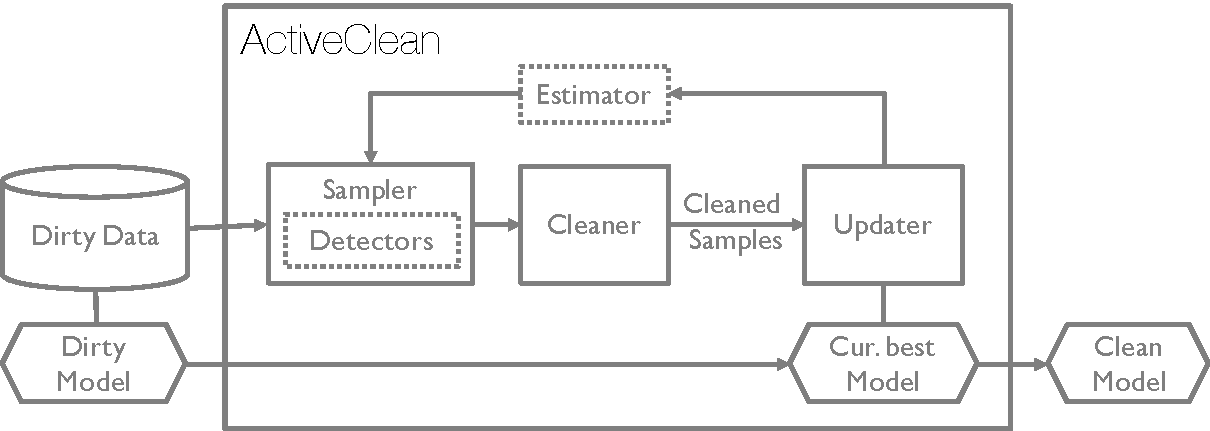
\includegraphics[width=0.8\columnwidth]{figs/arch.pdf}
 \caption{\sysfull (\sys) is an anytime framework from training models on dirty data. Expensive data transformations prior to model training are budgeted with a non-uniform sampling that priortizes examples that are most likely to change the model. As more data is cleaned the sampling distribution is updated.  \label{sys-arch}}
\end{figure}

\subsection{Example Use Case And API}
Consider the following example problem.
We are given the University of Texas Restaurant \footnote{http://www.cs.utexas.edu/users/ml/riddle/data/restaurant.tar.gz} dataset, which has the following schema:
\begin{lstlisting}[mathescape,basicstyle={\scriptsize}]
Restaurant(name$\textrm{,}$ address$\textrm{,}$ city$\textrm{,}$, type)
\end{lstlisting}
We want to train a Support Vector Machine classifier that given the tokens in the name and the city, can predict the category of the restaurant (e.g., Chinese or Mexican).
However, the challenge is that this dataset has numerous entity resolution problems where city names and categories are inconsistently represented.
\begin{lstlisting}[mathescape,basicstyle={\scriptsize}]
rex il ristorante,617 s. olive st.,los angeles,italian
rex il ristorante,617 s. olive st.,los angeles,nuova cucina italian
21 club,21 w. 52nd st.,new york,american
21 club,21 w. 52nd st.,new york city,american(new)
\end{lstlisting}
Entity resolution can be relatively expensive if the inconsistent representations are very different from each other and are not amenable to similarity measure optimizations such as prefix filtering or sorting.

\reminder{Maybe Describe API Here}

The analyst wants to quickly understand how much better a clean data set would be for this task.
Using our system, the analyst can construct a data cleaning workflow and specify a budget.
For example, this is what the code would look like in \sys.
\begin{lstlisting}[mathescape,basicstyle={\scriptsize}]
restaurant.load()

.clean(EntityResolution.weightedJaccard(`type',0.6))

.clean(EntityResolution.editDistance(`city',10))

.featureView(List(`type',`label'),(`city',`one_hot'),(`name',`bag_of_words')))

.model(new SVMModel(_))

.budget(5000)
\end{lstlisting}

\subsection{Algorithmic Problem Statement}
To formalize the optimization problem:

\noindent\textbf{Base Data and Featurization: } We are given a base dataset $\mathcal{R}$ which is a relation with $N$ rows. There is a featurization function $F$ which maps every row in $\mathcal{R}$ to a $d$ dimensional feature vector and a $l$ dimensional label tuple: \[F(r \in \mathcal{R}) \mapsto (\mathbb{R}^l, \mathbb{R}^d)\]. 

\noindent\textbf{Data Cleaning: } We define data cleaning as transformations that happens to the base data that result in changes to the feature vector. We do not consider data cleaning operations that change the number of rows in the relation such as row deletion or row deduplication. Allowed operations must result in the following changes to the feature vector: (1) feature transformation, (2) feature deletion, and (3) feature addition. Therefore, there is at most a one-to-one relationship beftween features in the cleaned data and the dirty data.

\reminder{Formalize Better}

\noindent\textbf{Budget Specification: } The analyst specifies two hyperparameters a cleaning budget $B$ which is the number of tuples to clean, and the number of cleaning rounds $T$. In each round, $\frac{B}{T}$ rows are processed by the system, we will discuss the tradeoffs between batching and incremental processing in the subsequent sections.

\reminder{Maybe exclude rounds}

\noindent\textbf{Model: } The analyst specifies the model which we require to be solved via convex regularized loss minimization:
\[
 \theta^{*}=\arg\min_{\theta}\sum_{i=1}^{N}\phi(x_{i},y_{i},\theta) + r(\theta)
\]

\noindent\textbf{Output: } The output of \sys is at each cleaning round we draw the sample of $\frac{B}{T}$ rows from a sampling distribution that incorporates information about the value of cleaning that row to model. After the $T$ cleaning rounds, the user is returned an approximately clean model $\theta^{(c)}$.
